% Compile from the repository root after creating tmp/pdfs:
%   pdflatex -output-directory=tmp/pdfs src/report.tex  (run twice)
%   or: tectonic --outdir tmp/pdfs src/report.tex
% Copy tmp/pdfs/report.pdf to report.pdf after compilation.
% Regenerate the column-width figure with: python src/PlotPaperFigures.py
\documentclass[10pt,twocolumn,letterpaper]{article}
\usepackage[margin=0.75in]{geometry}
\usepackage[T1]{fontenc}
\usepackage{lmodern,microtype}
\usepackage{amsmath,booktabs,graphicx}
\graphicspath{{./}{../}}
\usepackage{xcolor,enumitem,caption}
\usepackage[colorlinks=true,linkcolor=blue!40!black,urlcolor=blue!40!black,citecolor=blue!40!black]{hyperref}
\hypersetup{pdftitle={Fixed NULL Tokens for Arithmetic Learning: A Compute-Matched Evaluation},pdfauthor={Harvin Chhabra}}
\captionsetup{font=small,labelfont=bf,skip=5pt}
\setlength{\columnsep}{0.24in}
\setlength{\parindent}{1em}
\setlength{\parskip}{2pt}
\setlength{\textfloatsep}{12pt plus 2pt minus 2pt}
\setlength{\floatsep}{10pt plus 2pt minus 2pt}
\setlength{\emergencystretch}{1em}
\setlist{nosep,leftmargin=1.25em}
\newcommand{\nulltok}{\texttt{<NULL>}}
\begin{document}
\twocolumn[{
\begin{center}
{\LARGE\bfseries Fixed NULL Tokens for Arithmetic Learning:\\[3pt]
A Compute-Matched Evaluation\par}
\vspace{9pt}
{\large Harvin Chhabra}\\[3pt]
\href{mailto:harvinchhabra@gmail.com}{harvinchhabra@gmail.com}\\[3pt]
{\small October 2026}
\end{center}
\vspace{3pt}
\begin{center}\begin{minipage}{0.94\textwidth}
\small\textbf{Abstract.}
Additional sequence positions offer a simple way to allocate computation
before a language model commits to an answer. We study this approach in a
95K-parameter causal Transformer trained for integer addition, inserting four
learned NULL tokens before the answer with answer-only supervision. NULL
achieves 98.41\% exact-answer accuracy, compared with 95.48\% for the original
baseline and 96.57\% for a baseline trained from scratch at approximately the
same training FLOPs. The compute-matched comparison yields a 1.84
percentage-point gain and 53.6\% fewer exact-answer errors on 10,000 test
examples. Answer-token cross-entropy also decreases from 0.0259 to 0.0128.
Input ablations and longer-operand evaluations characterize the scope of this
effect. The results suggest that, within the tested distribution, allocating
computation through additional token positions can be more effective than
extending conventional baseline training.
\end{minipage}\end{center}
\vspace{12pt}
}]

\section{Introduction}
Intermediate tokens expand the representations available to a causal
Transformer before it generates an answer. Explicit scratchpads assign these
tokens readable computational steps; an alternative is to provide positions
without prescribing their semantic content. The motivation for this project
was to examine whether otherwise uninformative tokens could serve as a useful
computational workspace without written chain-of-thought supervision.

We investigate a minimal setting: character-level addition with a small
Transformer. The NULL variant receives four fixed tokens between the problem
and answer. We compare it with both an equal-duration baseline and a baseline
given additional training to match the estimated NULL compute budget.
This separates a simple accuracy comparison from the question of whether
spending that training budget on a conventional model recovers the gain.

The main result is a 1.84 percentage-point accuracy advantage over the
compute-matched baseline, corresponding to 184 additional correct answers
per 10,000 problems. We also evaluate dependence on the inserted tokens,
carry-count subgroups, and transfer to longer operands.

\section{Related Work}
Goyal et al.~\cite{goyal} introduce learnable pause tokens appended to language
model prefixes, with output extraction delayed until after the pauses.
Our fixed-NULL construction follows this general approach in a small arithmetic
setting, with an additional comparison against extended baseline training
under reconstructed training-compute budgets.

Pfau, Merrill, and Bowman~\cite{pfau} show that meaningless filler tokens can
support computation on algorithmic tasks under suitable supervision. Nye et
al.~\cite{nye} instead train language models to emit explicit intermediate
scratchpad steps, including for addition. Together, these studies motivate
examining the contribution of intermediate positions separately from written
reasoning content. Here, only answer characters and EOS are supervised.

Coconut~\cite{hao} explores continuous latent computation by feeding hidden
states back as subsequent input embeddings. In our implementation, each NULL
position receives a learned discrete-token embedding plus a positional
embedding. This provides a complementary, simpler construction using standard
causal Transformer inference.

\section{Experimental Setup}
\paragraph{Architecture and token insertion.}
Both models use two Transformer layers, width 72, four attention heads,
feedforward width 144, learned absolute positions, context length 128, no
dropout, and tied token/output embeddings. The baseline has 95,256 parameters;
adding NULL increases this to 95,328. Arithmetic is character-tokenized,
including spaces. The NULL prompt takes the form
\begin{center}\small
\texttt{12345 + 67890 = }\,$\nulltok^{\,4}$\,$\rightarrow$\,\texttt{80235 <EOS>}.
\end{center}
Four NULLs are inserted automatically after the complete problem prompt.
The model does not choose their number. NULL IDs are not supervised targets;
their representations receive gradients through the answer loss. Greedy
answer decoding forbids NULL, PAD, and UNK outputs.

\paragraph{Training.}
Original runs use 1,000,000 training rows, five epochs, batch size 64, AdamW
with learning rate $3\times10^{-4}$, gradient clipping at 1, and seed 42.
Original operands range from 0 to 99,999. All evaluations reuse the same
seed-42 sample of 10,000 rows from the million-row test file. Separate datasets
contain 10,000 unique ordered pairs of exactly six-digit and seven-digit
operands, generated with seeds 4206 and 4207 and Python-integer targets.

The primary metric is greedy exact-answer accuracy through EOS, with a
24-token generation cap and nontermination counted as incorrect. Answer-token
cross-entropy is token-weighted, includes EOS, and excludes the prompt and
inserted tokens. Each checkpoint uses its saved vocabulary.

\paragraph{Compute matching.}
For batch size $B$, padded length $L$, width $d$, layer count $N$, and vocabulary
size $V$, we estimate dense matrix-multiplication FLOPs as
\begin{align}
C_{\mathrm{fwd}} &= B\bigl[N(16Ld^2+4L^2d)+2LdV\bigr],\label{eq:flops}\\
C_{\mathrm{train}} &\approx 3C_{\mathrm{fwd}}.\nonumber
\end{align}
A multiply-add counts as two FLOPs. The terms cover attention projections,
feedforward layers of width $2d$, attention scores and weighted values, and
the output projection. We reconstruct the original batch order and maximum
padded lengths: 22 for baseline and 26 for NULL. Estimated step costs are
0.765794 and 0.917250 billion FLOPs, respectively, a 19.78\% difference.

The matched baseline is trained from scratch using the original seed,
initialization procedure, optimizer, learning rate, clipping, and shuffling.
Only its duration is extended. The target is the original five-epoch NULL
budget, matched to the nearest complete optimizer step (Table~\ref{tab:budget}).
The resulting mismatch is $-0.000268\%$. During its first five epochs, the
fresh baseline reproduces all 160 original loss-log entries within their
recorded four-decimal precision.

\begin{table}[t]
\centering\small
\setlength{\tabcolsep}{5pt}
\begin{tabular}{lrr}
\toprule
Model & Training steps & Training TFLOPs\\
\midrule
Baseline & 78,125 & 59.827680\\
NULL $\times4$ & 78,125 & 71.660160\\
Matched baseline & 93,576 & 71.659968\\
\bottomrule
\end{tabular}
\caption{Estimated training budgets. TFLOPs denotes $10^{12}$ operations.
The matched baseline processes 5,988,864 examples, versus 5,000,000 for each
original run.}\label{tab:budget}
\end{table}

\section{Results}
\subsection{Compute-matched accuracy}
Table~\ref{tab:accuracy} shows that extended baseline training improves
accuracy from 95.48\% to 96.57\%. NULL achieves 98.41\%, retaining a 1.84
percentage-point advantage at approximately equal training compute.
Its answer-token loss is 0.0128, compared with 0.0259 for the matched baseline.
Thus, both exact-answer accuracy and predictive loss favor the NULL model
under the matched budget.

\begin{table}[t]
\centering\small
\setlength{\tabcolsep}{4pt}
\begin{tabular}{lrrr}
\toprule
Model & Acc. (\%) & Loss & Errors\\
\midrule
Baseline & 95.48 & 0.0329 & 452\\
Matched baseline & 96.57 & 0.0259 & 343\\
\textbf{NULL $\times4$} & \textbf{98.41} & \textbf{0.0128} & \textbf{159}\\
\bottomrule
\end{tabular}
\caption{Original-distribution evaluation on 10,000 examples. Accuracy is
exact-answer accuracy; loss is answer-token cross-entropy.}\label{tab:accuracy}
\end{table}

The absolute accuracy difference represents a substantial change in residual
errors: NULL makes 159 errors instead of 343, a 53.6\% reduction relative to
the matched baseline (Figure~\ref{fig:errors}). Additional baseline training
therefore recovers part of the original gap, while the remaining difference
supports further investigation of how computation is allocated across
sequence positions. Carry-stratified results also favor NULL over the original
baseline in every observed carry-count group (0--5).

\begin{figure}[t]
\centering
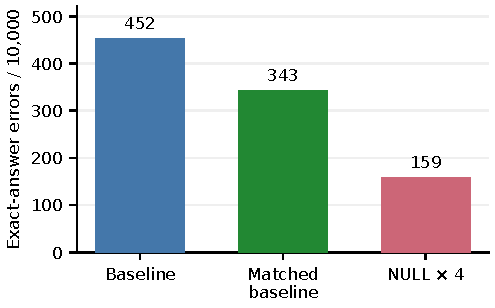
\includegraphics[width=\linewidth]{results/flop_matched/plots/paper/exact_answer_errors.pdf}
\caption{Exact-answer errors on the original-distribution test sample
(lower is better). NULL makes 184 fewer errors than the compute-matched
baseline, a relative reduction of 53.6\%.}\label{fig:errors}
\end{figure}

\subsection{Dependence on the inserted tokens}
Inference-only interventions preserve the NULL checkpoint and change its
prompt tokens (Table~\ref{tab:ablation}). Four NULLs achieve 98.41\% accuracy;
counts of 0, 1, 2, 3, or 8 yield 0\%. Replacing the four NULLs with UNK while
preserving length yields 1.52\%. These results establish a strong dependence
on the trained token configuration and motivate controls trained with
alternative tokens or variable counts.

\begin{table}[t]
\centering\small
\setlength{\tabcolsep}{8pt}
\begin{tabular}{lr}
\toprule
NULL-checkpoint input & Accuracy (\%)\\
\midrule
NULL $\times4$ (trained count) & 98.41\\
NULL $\times\{0,1,2,3,8\}$ & 0.00\\
UNK $\times4$ (same length) & 1.52\\
\bottomrule
\end{tabular}
\caption{Original-distribution input ablations without retraining.
Each count in the grouped row was evaluated separately.}\label{tab:ablation}
\end{table}

\subsection{Operand length and inference cost}
On both six- and seven-digit datasets, all three models score 0\% exact-answer
accuracy. The accuracy advantage is therefore specific to the original operand
range in these evaluations.

For original-distribution full-prefix generation without a KV cache, estimated
inference cost is 21.60 million FLOPs per problem for either baseline and
26.61 million for NULL (23.2\% more). This counts active generation through EOS,
excluding work on already-finished batch rows.

\section{Limitations}
\paragraph{Replication and scope.}
The study uses one initialization seed, one small architecture, and one task.
The observed accuracy and error reductions are descriptive; robustness across
seeds has not been established. Identical seeds also do not imply identical
shared-weight initializations when vocabulary sizes differ. Larger models,
additional tasks, and repeated runs are needed to assess transferability.

\paragraph{Mechanism and input distribution.}
The experiment does not identify the internal arithmetic procedure or test
the faithfulness of visible chains of thought. Four extra positions are
processed by the same two-layer network, rather than adding four layers or
guaranteeing four serial reasoning iterations. NULL allocation is externally
fixed; adaptive generation of thinking tokens is outside the present setup.
Ablating counts changes answer positions, while UNK replacement introduces an
untrained input pattern. These interventions cannot independently identify
embedding, positional, and computational effects.

\paragraph{Length extrapolation.}
No model generalizes successfully to the tested longer operands. Learned
absolute positions beyond the original training lengths are a possible
contributor, alongside changes in arithmetic length and token-position roles.
The current experiments do not distinguish these explanations. Length
curricula and positional-encoding comparisons would provide useful controls.

\paragraph{Compute estimates.}
Equation~\ref{eq:flops} counts full-square attention and approximates backward
cost as twice forward cost. It excludes normalization, softmax, activations,
biases, embedding lookup, optimizer operations, and memory traffic. Matching
this estimate does not match hardware time, energy, inference cost, or all
architectural differences. Inference estimates can also appear smaller for
OOD answers that terminate early, so they should be read with accuracy.

\paragraph{Data and evaluation coverage.}
Original train/test files share 97 exact expressions, or 187 test rows when
operand reversal is allowed. None of the exact overlaps occurs in the
10,000-row evaluation sample; reversed-pair overlap for this sample was not
separately reported. The original files contain duplicate rows. New longer
operand sets have disjoint ranges from training, but cover only two lengths
and one dataset seed per length.

\section{Conclusion}
Four fixed NULL tokens improve exact-answer accuracy in this small addition
model, reaching 98.41\% against 96.57\% for a compute-matched baseline. The
1.84 percentage-point gain corresponds to 53.6\% fewer errors and is supported
by lower answer-token loss. The result motivates studying token-based
allocation of computation alongside conventional increases in training
duration. Multi-seed replications, trained token controls, and adaptive
NULL-count policies are natural next steps.

\begin{thebibliography}{9}
\small
\bibitem{goyal} Sachin Goyal, Ziwei Ji, Ankit Singh Rawat, Aditya Krishna Menon,
Sanjiv Kumar, and Vaishnavh Nagarajan. \emph{Think before you speak: Training
Language Models With Pause Tokens}. ICLR, 2024; preprint, 2023.
\href{https://arxiv.org/abs/2310.02226}{arXiv:2310.02226}.
\bibitem{pfau} Jacob Pfau, William Merrill, and Samuel R. Bowman.
\emph{Let's Think Dot by Dot: Hidden Computation in Transformer Language
Models}. 2024. \href{https://arxiv.org/abs/2404.15758}{arXiv:2404.15758}.
\bibitem{nye} Maxwell Nye et al. \emph{Show Your Work: Scratchpads for
Intermediate Computation with Language Models}. 2021.
\href{https://arxiv.org/abs/2112.00114}{arXiv:2112.00114}.
\bibitem{hao} Shibo Hao, Sainbayar Sukhbaatar, DiJia Su, Xian Li, Zhiting Hu,
Jason Weston, and Yuandong Tian. \emph{Training Large Language Models to
Reason in a Continuous Latent Space}. Preprint, 2024; COLM, 2025.
\href{https://arxiv.org/abs/2412.06769}{arXiv:2412.06769}.
\end{thebibliography}

\paragraph{Reproducibility.}
Source code, metrics, dataset audits, and compute-method reports accompany
this paper in the repository. The paper uses the saved experiment outputs;
no new training or evaluation was performed for this revision.
\end{document}
